\documentclass[12pt]{../style-files/ociamthesis}

\usepackage{amssymb}
\usepackage{titlesec}
\usepackage{amsmath}
\usepackage{float}
\usepackage{graphicx}
\usepackage{caption}
\usepackage{subfig}
\usepackage{xcolor}
\usepackage[section]{placeins}
\usepackage{mathrsfs}
\usepackage{bm}
\usepackage{stmaryrd}
\usepackage{siunitx}
\usepackage{rotating}
\usepackage[utf8]{inputenc}
\usepackage[round]{natbib}
\usepackage{tikz}
\usetikzlibrary{fadings}
\usetikzlibrary{snakes}

%%%%%%%%%%%%%%%%%%%%%%%%%%%%%%%%%%%%%%%%%%%%%%%%%%%%%%%%%%
% the following is to alter tikz settings to improve springs figure.
\usetikzlibrary{decorations.pathmorphing,calc,patterns}
\makeatletter
\def\pgfdecorationspringstraightlinelength{0.5cm}
\def\pgfdecorationspringnumberofelement{8}
\def\pgfdecorationspringnaturallength{5cm}
\pgfkeys{%
	/pgf/decoration/.cd,
	spring straight line length/.code={%
		\pgfmathsetlengthmacro\pgfdecorationspringstraightlinelength{#1}},
	spring natural length/.code={%
		\pgfmathsetlengthmacro\pgfdecorationspringnaturallength{#1}},
	spring number of element/.store in=\pgfdecorationspringnumberofelement
}

\pgfdeclaredecoration{coil spring}{straight line}{%
	\state{straight line}[%
	persistent precomputation = {%
		% Compute the effective length of the spring (without the length
		% of the two straight lines): \pgfdecorationspringeffectivelength
		\pgfmathsetlengthmacro{\pgfdecorationspringeffectivelength}%
		{\pgfdecoratedpathlength-2*\pgfdecorationspringstraightlinelength}
		% Compute the effective length of one coil pattern:
		% \pgfdecorationspringeffectivelengthofonecoil
		\pgfmathsetlengthmacro{\pgfdecorationspringeffectivelengthofonecoil}%
		{\pgfdecorationspringeffectivelength/\pgfdecorationspringnumberofelement}
	},
	width = \pgfdecorationspringstraightlinelength,
	next state = draw spring]{%
		\pgfpathlineto{%
			\pgfqpoint{%
				\pgfdecorationspringstraightlinelength}{0pt}}
	}
	\state{draw spring}%
	[width=\pgfdecorationspringeffectivelengthofonecoil,
	repeat state=\pgfdecorationspringnumberofelement-1,next state=final]{%
		\pgfpathcurveto
		{\pgfpoint@onspringcoil{0    }{ 0.555}{1}}
		{\pgfpoint@onspringcoil{0.445}{ 1    }{2}}
		{\pgfpoint@onspringcoil{1    }{ 1    }{3}}
		\pgfpathcurveto
		{\pgfpoint@onspringcoil{1.555}{ 1    }{4}}
		{\pgfpoint@onspringcoil{2    }{ 0.555}{5}}
		{\pgfpoint@onspringcoil{2    }{ 0    }{6}}
		\pgfpathcurveto
		{\pgfpoint@onspringcoil{2    }{-0.555}{7}}
		{\pgfpoint@onspringcoil{1.555}{-1    }{8}}
		{\pgfpoint@onspringcoil{1    }{-1    }{9}}
		\pgfpathcurveto
		{\pgfpoint@onspringcoil{0.445}{-1    }{10}}
		{\pgfpoint@onspringcoil{0    }{-0.555}{11}}
		{\pgfpoint@onspringcoil{0    }{ 0    }{12}}
	}
	\state{final}{%
		\pgfpathlineto{\pgfpointdecoratedpathlast}
	}
}

\def\pgfpoint@onspringcoil#1#2#3{%
	\pgf@x=#1\pgfdecorationsegmentamplitude%
	\pgf@x=.5\pgf@x%
	\pgf@y=#2\pgfdecorationsegmentamplitude%
	\pgfmathparse{0.083333333333*\pgfdecorationspringeffectivelengthofonecoil}%
	\pgf@xa=\pgfmathresult pt
	\advance\pgf@x by#3\pgf@xa%
}

\makeatother

\tikzset{%
	Spring/.style = {%
		decoration = {%
			coil spring,
			spring straight line length = 0.2cm,
			% To be added
			spring natural length = #1,
			spring number of element = 4,
			amplitude=2mm},
		decorate,
		very thick},
	Spring/.default = {4cm}}
%%%%%%%%%%%%%%%%%%%%%%%%%%%%%%%%%%%%%%%%%%%%%%%%%


\usepackage{geometry}
 \geometry{
 a4paper,
 left=40mm,
 right=30mm,
 top=30mm,
 bottom=30mm
 }

\definecolor{theblue}{HTML}{0000CD}

% disable this package for printed version
\usepackage[colorlinks=true, linktocpage=true, allcolors=theblue]{hyperref}

\titleformat{\chapter}[display]
  {\bfseries\Large}
  {\filright\MakeUppercase{\chaptertitlename} \Large\thechapter}
  {1ex}
  {}
  [\vspace{1ex} \hrule \vspace{1pt} \hrule]

\newcommand{\adv}{    {\it Adv. Space Res.}} 
\newcommand{\annG}{   {\it Ann. Geophys.}} 
\newcommand{\aap}{    {\it Astron. Astrophys.}}
\newcommand{\aaps}{   {\it Astron. Astrophys. Suppl.}}
\newcommand{\aapr}{   {\it Astron. Astrophys. Rev.}}
\newcommand{\ag}{     {\it Ann. Geophys.}}
\newcommand{\aj}{     {\it Astron. J.}} 
\newcommand{\apj}{    {\it Astrophys. J.}}
\newcommand{\apjl}{   {\it Astrophys. J. Lett.}}
\newcommand{\apss}{   {\it Astrophys. Space Sci.}} 
\newcommand{\cjaa}{   {\it Chin. J. Astron. Astrophys.}} 
\newcommand{\gafd}{   {\it Geophys. Astrophys. Fluid Dyn.}}
\newcommand{\grl}{    {\it Geophys. Res. Lett.}}
\newcommand{\ijga}{   {\it Int. J. Geomagn. Aeron.}}
\newcommand{\jastp}{  {\it J. Atmos. Solar-Terr. Phys.}} 
\newcommand{\jgr}{    {\it J. Geophys. Res.}}
\newcommand{\mnras}{  {\it Mon. Not. Roy. Astron. Soc.}}
\newcommand{\na}{     {\it New Astronomy}}
\newcommand{\nat}{    {\it Nature}}
\newcommand{\pasp}{   {\it Pub. Astron. Soc. Pac.}}
\newcommand{\pasj}{   {\it Pub. Astron. Soc. Japan}}
\newcommand{\pre}{    {\it Phys. Rev. E}}
\newcommand{\solphys}{{\it Solar Phys.}}
\newcommand{\sovast}{ {\it Soviet  Astron.}} 
\newcommand{\ssr}{    {\it Space Sci. Rev.}}
\newcommand{\caa}{    {\it Chinese Astron. Astrohpys.}} 
\newcommand{\apjs}{   {\it Astrophys. J. Suppl.}}

\begin{document}

\baselineskip=18pt

\setcounter{secnumdepth}{3}
\setcounter{tocdepth}{3}

\setcounter{chapter}{1}


\newcommand{\bv}{\mathbf{v}}
\newcommand{\bB}{\mathbf{B}}


%------------------------------------------------------------------------------
\chapter{Asymmetric waveguides - eigenvalue problem}
\label{chap: EVP}
%------------------------------------------------------------------------------

The simplest model of an asymmetric waveguide is an asymmetric magnetic slab in a non-magnetic environment\footnote{More precisely, the simplest model of an asymmetric MHD waveguide is an interface between different plasmas; the asymmetric slab is the simplest asymmetric waveguide that can oscillate in a collective body mode (see Section~\ref{sec: body}).}

%------------------------------------------------------------------------------
\section{Chapter introduction}
\label{sec: EVP intro}
%------------------------------------------------------------------------------

Section~\ref{sec: EVP non-mag} is based on \cite{all_etal17} and Section~\ref{sec: EVP mag} is based on \cite{zsa_etal18}.

%------------------------------------------------------------------------------
\section{Asymmetric slab}
\label{sec: asym slab}
%------------------------------------------------------------------------------
\subsection{Model description}
Figure~\ref{fig:eq} illustrates the construction of this mathematical model, where a three-dimensional, unbounded, inviscid plasma is separated into three regions by two parallel planar interfaces at $x = \pm x_0$. The equilibrium magnetic field is in the $z$-direction and has magnitude
\begin{equation}
	B(x)=
	\begin{cases}
		B_1 & \text{if } x < -x_0, \\
		B_0 & \text{if } |x|\leq{x_0}, \\
		B_2 & \text{if } x > x_0,
	\end{cases}
\end{equation}
where $B_j$, for $j = 0, 1, 2$ are constant. Within each region, denoted by subscripts 0, 1, and 2, the plasma is uniform and the equilibrium plasma pressure, density, and temperature are denoted by $p_j$, $\rho_j$, and $T_j$, respectively, for $j = 0, 1, 2$. This defines an \textit{isolated} waveguide, by which we mean there is no adjacent waveguides that can effect the oscillations.

\begin{figure}
	\centering
	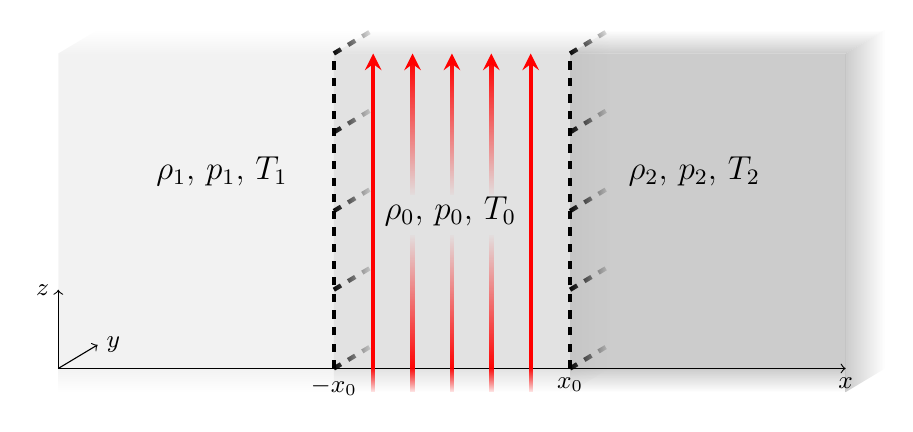
\begin{tikzpicture}
	\path [fill=lightgray, opacity=0.45] (3.5,0) -- (3.5,4) -- (6.5,4) -- (6.5,0) -- (3.5,0);
	\shade[left color=lightgray,right color=white, opacity=0.45] (6.5,0) -- (6.5,4) -- (7,4.3) -- (7,0.3) -- (6.5,0);
	\shade[top color=lightgray,bottom color=white, opacity=0.45] (3.5,0) -- (6.5,0) -- (6.5,-0.3) -- (3.5,-0.3) -- (3.5,0);
	\shade[top color=white,bottom color=lightgray, opacity=0.45] (3.5,4) -- (4,4.3) -- (7,4.3) -- (6.5,4) -- (3.5,4);
	\shade[left color=lightgray,right color=white, opacity=0.45] (6.5,0) -- (6.5,-0.3) -- (7,0) -- (7,0.3) -- (6.5,0);
	
	\path [fill=lightgray, opacity=0.8] (6.5,0) -- (6.5,4) -- (10,4) -- (10,0) -- (6.5,0);
	\shade[top color=lightgray,bottom color=white, opacity=0.8] (6.5,0) -- (10,0) -- (10,-0.3) -- (6.5,-0.3) -- (6.5,0);
	\shade[top color=white,bottom color=lightgray, opacity=0.8] (6.5,4) -- (7,4.3) -- (10.5,4.3) -- (10,4) -- (6.5,4);
	\shade[left color=lightgray,right color=white, opacity=0.8] (10,-0.3) -- (10,4) -- (10.5,4.3) -- (10.5,0) -- (10,-0.3);
	
	\path [fill=lightgray, opacity=0.2] (0,0) -- (0,4) -- (3.5,4) -- (3.5,0) -- (0,0);
	\shade[top color=lightgray,bottom color=white, opacity=0.2] (0,0) -- (3.5,0) -- (3.5,-0.3) -- (0,-0.3) -- (0,0);
	\shade[top color=white,bottom color=lightgray, opacity=0.2] (0,4) -- (0.5,4.3) -- (4,4.3) -- (3.5,4) -- (0,4);
	
	\draw [<->] (0,1) -- (0,0) -- (10,0);
	\draw [->] (0,0) -- (0.5,0.3);
	
	\draw [ultra thick, dashed] (3.5,0) -- (3.5,4);
	\draw [ultra thick, dashed, path fading=east] (3.5,0) -- (4,0.3);
	\draw [ultra thick, dashed, path fading=east] (3.5,4) -- (4,4.3);
	\draw [ultra thick, dashed, path fading=east] (3.5,2) -- (4,2.3);
	\draw [ultra thick, dashed, path fading=east] (3.5,1) -- (4,1.3);
	\draw [ultra thick, dashed, path fading=east] (3.5,3) -- (4,3.3);
	\draw [ultra thick, red, -stealth] (4,0) -- (4,4);
	\draw [ultra thick, red, path fading=south] (4,-0.3) -- (4,0);
	\draw [ultra thick, red, path fading=north] (4.5,0) -- (4.5, 1.7);
	\draw [ultra thick, red, path fading=south] (4.5,-0.3) -- (4.5,0);
	\draw [ultra thick, red, path fading=south] (4.5,2.2) -- (4.5,3.9);
	\draw [ultra thick, red, -stealth] (4.5,3.9) -- (4.5,4);
	\draw [ultra thick, red, path fading=north] (5,0) -- (5, 1.7);
	\draw [ultra thick, red, path fading=south] (5,-0.3) -- (5, 0);
	\draw [ultra thick, red, path fading=south] (5,2.2) -- (5,3.9);
	\draw [ultra thick, red, -stealth] (5,3.9) -- (5,4);
	\draw [ultra thick, red, path fading=north] (5.5,0) -- (5.5, 1.7);
	\draw [ultra thick, red, path fading=south] (5.5,-0.3) -- (5.5, 0);
	\draw [ultra thick, red, path fading=south] (5.5,2.2) -- (5.5,3.9);
	\draw [ultra thick, red, -stealth] (5.5,3.9) -- (5.5,4);
	\draw [ultra thick, red, -stealth] (6,0) -- (6,4);
	\draw [ultra thick, red, path fading=south] (6,-0.3) -- (6,0);
	\draw [ultra thick, dashed] (6.5,0) --(6.5,4);
	\draw [ultra thick, dashed, path fading=east] (6.5,0) -- (7,0.3);
	\draw [ultra thick, dashed, path fading=east] (6.5,4) -- (7,4.3);
	\draw [ultra thick, dashed, path fading=east] (6.5,2) -- (7,2.3);
	\draw [ultra thick, dashed, path fading=east] (6.5,1) -- (7,1.3);
	\draw [ultra thick, dashed, path fading=east] (6.5,3) -- (7,3.3);
	
	\small
	\node [below] at (3.5,0) {$-x_0$};
	\node [below] at (6.5,0) {$x_0$};
	\node [below] at (10,0) {$x$};
	\node [left] at (0,1) {$z$};
	\node [right] at (0.5,0.3) {$y$};
	
	\large
	\node [right] at (1.1,2.5) {$\rho_1$, $p_1$, $T_1$};
	\node [right] at (4,2) {$\rho_0$, $p_0$, $T_0$};
	\node [right] at (7.1,2.5) {$\rho_2$, $p_2$, $T_2$};
	\end{tikzpicture}
	\caption{The equilibrium state inside the slab, ($|x| \leq x_0$) and outside the slab, ($x < -x_0$ and $x > x_0$). The red arrows illustrate magnetic field lines, $B(x)\mathbf{\widehat{z}}$, and the dashed black lines indicate the boundaries of the slab. \textcolor{red}{Change to mag outside}}
	\label{fig:eq}
\end{figure}

To ensure that the model is in equilibrium, the total pressure in each external region must balance the total pressure in the internal region, namely
\begin{equation}
	p_1 + \frac{B_1^2}{2\mu_0} = p_0 + \frac{B_0^2}{2\mu_0} = p_2 + \frac{B_2^2}{2\mu_0}, \label{pressure balance}
\end{equation}
where $\mu_0$ is the permeability of free space. We can rewrite Equation~\eqref{pressure balance} as
\begin{equation}
\rho_i\left(c_i^2 + \frac{\gamma}{2}v_{Ai}^2\right) = \rho_j\left(c_j^2 + \frac{\gamma}{2}v_{Aj}^2\right), \quad \text{for} \quad i, j = 0, 1, 2, \label{sound speeds}
\end{equation}
where we define the sound and Alfv\'{e}n speeds in each region by $c_j = \sqrt{\gamma p_j/\rho_j}$ and $v_{Aj} = B_j/\sqrt{\mu\rho_j}$, respectively, for $j = 0, 1, 2$. The adiabatic index\footnote{The adiabatic index is assumed uniform across the whole domain under the single-fluid approximation.} is $\gamma$.


\subsection{The dispersion relation}

In the derivation of the dispersion relation, we decompose the linearised ideal MHD equations into Fourier forms then combine them into an ordinary differential equation (ODE) for the transverse velocity perturbation for each of the three plasma regions. After finding the general solution to each of these ODEs, we match the solutions across each interface at $\pm x_0$. The condition for the existence of non-trivial solutions will lead to the dispersion relation. In mathematical terms, we're converting a set of partial differential equations into ordinary differential equations into algebraic equations, into a single equation. From a form that we cannot solve into a form that we can.


\subsubsection{Derivation} \label{sec: asym slab DR der}

We begin with the ideal MHD equations, linearised around a static equilibrium with subscripts $j$, Equations~\eqref{cont eqn lin}-\eqref{ind eqn lin}. Taking the partial derivative with respect to time of Equation~\eqref{mom eqn lin} and eliminating $bB$ using Equation~\eqref{ind eqn lin}, gives
\begin{align}
	\frac{\partial^2 v_x}{\partial t^2} &= \frac{\partial}{\partial x}\left[ (c_j^2 + v_{Aj}^2)\nabla\cdot\bv - v_{Aj}^2\frac{\partial v_z}{\partial z} \right] + v_{Aj}^2 \frac{\partial^2 v_x}{\partial z^2} \label{mom x} \\
	\frac{\partial^2 v_y}{\partial t^2} &= \frac{\partial}{\partial y}\left[ (c_j^2 + v_{Aj}^2)\nabla\cdot\bv - v_{Aj}^2\frac{\partial v_z}{\partial z} \right] + v_{Aj}^2 \frac{\partial^2 v_y}{\partial z^2} \label{mom y} \\
	\frac{\partial^2 v_z}{\partial t^2} &= c_j^2\frac{\partial}{\partial z}(\nabla\cdot\bv). \label{mom z}
\end{align}
Now we seek solutions of the Fourier form
\begin{equation}
\bv(\mathbf{x},t)=(\hat{v}_x(x)\textrm{e}^{i(kz-\omega{t})}, 0, \hat{v}_z(x)\textrm{e}^{i(kz-\omega{t})}),
\label{vcomponents}
\end{equation}
where $\mathbf{k} = (0, 0, k)$ is the wavenumber vector and $\omega$ is the angular frequency. This restricts the investigation to waves propagating parallel to the equilibrium magnetic field, with velocity perturbation amplitude $\hat{v}_x(x)$ in the $x$-direction, and $\hat{v}_z(x)$ in the $z$-direction. With this ansatz, Equation~\eqref{mom y} degenerates and Equations~\eqref{mom x} and~\eqref{mom z} become
\begin{align}
&-\omega^2\hat{v}_x = (c_j^2+v_\textrm{Aj}^2)(\hat{v}_x'' + ik\hat{v}_z') - v_\textrm{Aj}^2ik\hat{v}_z'-v_\textrm{Aj}^2k^2\hat{v}_x, \label{mom x 2} \\
&-\omega^2\hat{v}_z = c_j^2ik(\hat{v}_x' + ik\hat{v}_z), \label{mom z 2}
\end{align}
where $' = d/dx$. These equations can be combined to give an ordinary differential equation for $\hat{v}_x$, namely
\begin{equation}
\hat{v}_x'' - m_j^2\hat{v}_x = 0, \quad \text{where} \quad
m_j^2 = \frac{(k^2v_\textrm{Aj}^2 - \omega^2)(k^2c_j^2 - \omega^2)}{(c_j^2 + v_\textrm{Aj}^2)(k^2c_\textrm{Tj}^2 - \omega^2)}. \label{O}
\end{equation}
This is identical to the corresponding equation governing, for example, a tangential interface or a symmetric slab, derived in Sections~\ref{sec: MHD waves interface} and~\ref{sec: MHD waves sym slab} by \cite{rob81a,rob81c}.

Solutions of Equations~\eqref{O} are a linear combination of hyperbolic functions. We restrict our model to waves trapped by the slab by imposing the boundary condition $\hat{v}_x \to 0$ as $|x| \to \infty$. Thus, the general solution for the velocity perturbation in the $x$-direction is
\begin{equation}
\hat{v}_x(x)=
\begin{cases}
A(\cosh{m_1x} + \sinh{m_1x}), & \text{if } x < -x_0, \\
B\cosh{m_0x} + C\sinh{m_0x}, & \text{if } |x| \leq {x_0}, \\
D(\cosh{m_2x} - \sinh{m_2x}), & \text{if  } x > x_0, 
\end{cases} \label{vsoln}
\end{equation}
where $A$, $B$, $C$, and $D$ are arbitrary constants (with respect to $x$). The remaining boundary conditions are continuity of velocity and total pressure across the slab boundaries at $x = \pm{x_0}$. With the aim of finding an expression for the total pressure perturbation, the Equations~\eqref{cont eqn lin} and~\eqref{energy eqn lin} can be combined to give
\begin{equation}
	\frac{\partial p}{\partial t} = - \rho_jc_i^2\nabla\cdot\bv.
\end{equation}
Using the above equation and the $z$-component of Equation~\eqref{ind eqn lin}, the perturbation in total pressure (plasma pressure, $p$, plus magnetic pressure, $B_jB_z/\mu$) across the whole domain can be shown to have amplitude
\begin{equation}
\hat{p}_T(x) = \frac{\Lambda_j}{m_j}\hat{v}_x'(x),
\end{equation}
where
\begin{equation}
\Lambda_j = \frac{i\rho_j(\omega^2 - \omega_{Aj}^2)}{m_j\omega}, \quad \text{for} \quad j = 0, 1, 2. \label{Lambdas}
\end{equation}
Ensuring continuity of velocity and total pressure across the slab boundaries gives four coupled algebraic equations, namely
\begin{equation}
\left(
\begin{matrix}
c_1-s_1             &-c_0           &s_0            &0                   \\
0                   &c_0            &s_0            &s_2-c_2             \\
\Lambda_1(c_1-s_1)  &\Lambda_0s_0   &-\Lambda_0c_0  &0                   \\
0                   &\Lambda_0s_0   &\Lambda_0c_0   &-\Lambda_2(s_2-c_2)
\end{matrix}
\right)
\left(
\begin{matrix}
A \\
B \\
C \\
D
\end{matrix}
\right)
=
\left(
\begin{matrix}
0 \\
0 \\
0 \\
0
\end{matrix}
\right),
\label{coefmatrix}
\end{equation}
where $c_j = \cosh{m_jx_0}$ and $s_j = \sinh{m_jx_0}$ for $j=0,1,2$, for brevity. The condition for the existence of non-trivial solutions to this system of equations is that the determinant of the matrix is zero. Applying this condition gives us the dispersion relation for an asymmetric slab, namely
\begin{equation}
(\Lambda_0^2 + \Lambda_1\Lambda_2) + \Lambda_0(\Lambda_1 + \Lambda_2)\coth{2m_0x_0} = 0. \label{DR lambda}
\end{equation}
By expanding each $\Lambda_j$, we can write this dispersion relation in familiar variables as
\begin{align}
&m_0^2(\omega^2 - \omega_{A1}^2)(\omega^2 - \omega_{A2}^2) + \frac{\rho_0}{\rho_1}m_1\frac{\rho_0}{\rho_2}m_2(\omega^2 - \omega_{A0}^2)^2 \notag \\
& + m_0(\omega^2 - \omega_{A0}^2)\left[\frac{\rho_0}{\rho_1}m_1(\omega^2 - \omega_{A2}^2) + \frac{\rho_0}{\rho_2}m_2(\omega^2 - \omega_{A1}^2)\right]\coth{2m_0x_0} = 0. \label{DR}
\end{align}


\subsubsection{First-order asymmetric slab}

There is a qualitative difference between waves propagating along symmetric and asymmetric magnetic slabs. The dispersion relation governing an asymmetric slab is a single equation, whereas the dispersion relation governing a symmetric slab \citep{rob81a} consists of two independent equations, corresponding to the sausage and kink eigenmodes.

Under the approximation that the densities and temperatures of the external plasma are of the same order, the dispersion relation, Equation~\eqref{DR}, can be factorised to give the approximate dispersion relation
\begin{equation}
\left[\Lambda_0(\Lambda_1+\Lambda_2)+2\Lambda_1\Lambda_2\tanh{m_0x_0}\right]\left[\Lambda_0(\Lambda_1+\Lambda_2)+2\Lambda_1\Lambda_2\coth{m_0x_0}\right]=0. \label{DR approx lambda}
\end{equation}
To show this, define each bracket as the following functions
\begin{align}
D_s(\omega) &:= \Lambda_0(\Lambda_1 + \Lambda_2) + 2\Lambda_1\Lambda_2\tanh{m_0x_0}, \\
D_k(\omega) &:= \Lambda_0 (\Lambda_1 + \Lambda_2) + 2\Lambda_1\Lambda_2\coth{m_0x_0}.
\end{align}
There product is
\begin{align}
D_s(\omega)D_k(\omega) &= \left[ \Lambda_0(\Lambda_1 + \Lambda_2) + 2\Lambda_1\Lambda_2\tanh{m_0x_0} \right] \left[ \Lambda_0 (\Lambda_1 + \Lambda_2) + 2\Lambda_1\Lambda_2\coth{m_0x_0} \right] \\
&= \Lambda_0^2 (\Lambda_1 + \Lambda_2)^2 + 2\Lambda_0(\Lambda_1 + \Lambda_2)\Lambda_1\Lambda_2(\tanh{m_0x_0} + \coth{m_0x_0}) + 4\Lambda_1^2\Lambda_2^2 \\
&= 4\Lambda_1\Lambda_2 \left[ (\Lambda_0^2F + \Lambda_1\Lambda_2) + \Lambda_0(\Lambda_1 + \Lambda_2)\coth(2m_0x_0) \right] \\
\end{align}
where
\begin{equation}
F = \frac{(\Lambda_1 + \Lambda_2)^2}{4\Lambda_1\Lambda_2}.
\end{equation}
When the plasma parameters on each side of the slab are approximately equal, \textit{i.e.} $\Lambda_2 = \Lambda_1 (1 + \epsilon L)$, with $\epsilon \ll 1$ and $L \approx 1$, $F$ becomes
\begin{equation}
F = \frac{(2 + \epsilon L)^2}{4(1 + \epsilon L)} = 1 + \mathcal{O}(\epsilon^2).
\end{equation}
Therefore, 
\begin{equation}
(\Lambda_0^2 + \Lambda_1\Lambda_2) + \Lambda_0(\Lambda_1 + \Lambda_2)\coth(2m_0x_0) = \frac{1}{4\Lambda_1\Lambda_2} D_s(\omega) D_k(\omega) + \mathcal{O}(\epsilon^2).
\end{equation}
Therefore, to linear order of waveguide asymmetry, if the dispersion relation, Equation~\eqref{DR lambda} is satisfied, then either $D_s(\omega) = 0$ or $D_k(\omega) = 0$, which completes the proof of Equation~\eqref{DR approx lambda}.

The expressions for the variables $\Lambda_i$ for $i=0,1,2$ in Equations~\eqref{Lambdas} can be employed to yield the approximately symmetric dispersion relation
\begin{equation}
(\omega^2 - \omega_{A0}^2)\left(\frac{\rho_0}{\rho_1}\frac{m_1}{(\omega^2 - \omega_{A1}^2)} + \frac{\rho_0}{\rho_2}\frac{m_2}{(\omega^2 - \omega_{A2}^2)}\right) + 2m_0\left(\begin{matrix}\tanh \\ \coth \end{matrix}\right)(m_0x_0) = 0. \label{DRapprox}
\end{equation}
This equation is now in a form similar to Equation~\eqref{DR sym slab}, the dispersion relation corresponding to MHD waves along a symmetric magnetic slab (Section~\ref{sec: MHD waves sym slab}), namely
\begin{equation}
\rho_im_e(\omega^2 - \omega_\textrm{Ai}^2) + \rho_em_i(\omega^2 - \omega_\textrm{Ae}^2)\left(\begin{matrix}\tanh \\ \coth \end{matrix}\right)(m_ix_0) = 0, \label{DRsym}
\end{equation}
where internal and external parameters are denoted by subscripts $i$ and $e$.


\subsection{Asymmetric eigenmodes}
There is a rich spectrum of MHD eigenmodes on a magnetic slab. In a symmetric slab, the dispersion relation, Equation~\eqref{DRsym}, consists of two decoupled equations that correspond to the two types of fundamental wave supported by the slab: the ``sausage" and ``kink" MHD waves.

\textit{Similar to waves in a symmetric slab (Section~\ref{sec: MHD wvaes sym slab}), waves for which $m_0^2 > 0$ correspond to exponential solutions of Equation~\eqref{vsoln} within the slab, known as surface waves. Waves for which $m_0^2 < 0$ correspond to trigonometric solutions of Equation~\eqref{vsoln} within the slab, known as body waves.}

Sausage and kink modes can be further categorised into ``surface" and ``body" modes. Surface modes are waves more enhanced at the slab boundaries, whereas body waves are characterised by oscillations permeating spatially throughout the slab, having their maximum amplitude within the slab. Mathematically, surface waves correspond to exponential solutions of Equation~\eqref{O}, that is, they exist when $m_0^2>0$, which occurs when the phase speed $\omega/k$ satisfies
\begin{equation}
\frac{\omega}{k}<c_\textrm{T} \quad \text{or} \quad \text{min}\{c_0, v_\textrm{A}\}<\frac{\omega}{k}<\text{max}\{c_0, v_\textrm{A}\}.
\end{equation}
Body waves correspond to spatially oscillatory solutions (\textit{i.e.} they can have nodes inside the slab), that is, they exist when $m_0^2<0$, which occurs when
\begin{equation}
c_\textrm{T}<\frac{\omega}{k}<\text{min}\{c_0, v_\textrm{A}\} \quad \text{or} \quad \text{max}\{c_0, v_\textrm{A}\}<\frac{\omega}{k}. \label{bconditions}
\end{equation}

For an asymmetric slab, the sausage and kink modes are modified by the external density difference, causing an asymmetry of the oscillation amplitude on each side of the slab (for visualisation see Figures~\ref{fig:saus} and~\ref{fig:kink}). We call these asymmetric eigenmodes quasi-sausage and quasi-kink modes. In a symmetric slab, sausage modes are characterised by a line of zero perturbation at the centre of the slab. In an asymmetric slab, this line is shifted towards the side of greatest external density. For symmetric kink modes, the width of the perturbed slab remains constant along the slab, but this characteristic is dropped in an asymmetric slab. This highlights the mixed nature of these modes.

\begin{figure}
	\makebox[\textwidth][c]{
		\subfloat[Quasi-kink]{\scalebox{1}{
				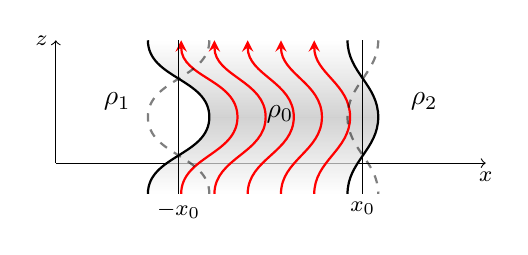
\begin{tikzpicture}[scale=0.78]
				\draw [->] (0,0) -- (7,0);
				
				\shade[bottom color=lightgray,top color=white, opacity=0.7] (1.5,2) to [out=-90,in=90] (2.5,0.75) to (5.25,0.75) to [out=90,in=-90] (4.75,2) to (1.5,2);
				
				\shade[bottom color=white,top color=lightgray, opacity=0.7] (2.5,0.75) to (5.25,0.75) to [out=-90,in=90] (4.75,-0.5) to (1.5,-0.5) to [out=90,in=-90] (2.5,0.75);
				
				\draw [thick] (1.5,2) to [out=-90,in=90] (2.5,0.75) to [out=-90,in=90] (1.5,-0.5);
				\draw [thick] (4.75,2) to [out=-90,in=90] (5.25,0.75) to [out=-90,in=90] (4.75,-0.5);
				
				\draw [thick, red, -stealth] (2.0417,-0.5) to [out=90,in=-90] (2.9583, 0.75) to [out=90,in=-90] (2.0417,2);
				\draw [thick, red, -stealth] (2.5833,-0.5) to [out=90,in=-90] (3.4167, 0.75) to [out=90,in=-90] (2.5833,2);
				\draw [thick, red, -stealth] (3.125,-0.5) to [out=90,in=-90] (3.875, 0.75) to [out=90,in=-90] (3.125,2);
				\draw [thick, red, -stealth] (3.6667,-0.5) to [out=90,in=-90] (4.3333, 0.75) to [out=90,in=-90] (3.6667,2);
				\draw [thick, red, -stealth] (4.2083,-0.5) to [out=90,in=-90] (4.7917, 0.75) to [out=90,in=-90] (4.2083,2);
				
				\draw [thick, dashed, opacity=0.5] (2.5,2) to [out=-90,in=90] (1.5,0.75) to [out=-90,in=90] (2.5,-0.5);
				\draw [thick, dashed, opacity=0.5] (5.25,2) to [out=-90,in=90] (4.75,0.75) to [out=-90,in=90] (5.25,-0.5);
				
				% % % % % % % % % % % % % % % % % % % % % % % % % %
				
				\draw [->] (0,0) -- (0,2);
				
				\node at (1,1) {$\rho_1$};
				\node at (6,1) {$\rho_2$};
				\node at (3.65,0.8) {$\rho_0$};
				
				\footnotesize
				\node [below] at (2,-0.5) {$-x_0$};
				\node [below] at (5,-0.5) {$x_0$};
				
				\node [left] at (0,2) {$z$};
				\node [below] at (7,0) {$x$};
				\draw [-] (2,-0.5) -- (2,2);
				\draw [-] (5,-0.5) -- (5,2);
				\end{tikzpicture}
				\label{fig:saus}}}
		%
		%
		%
		%
		\subfloat[Quasi-sausage]{\scalebox{1}{
				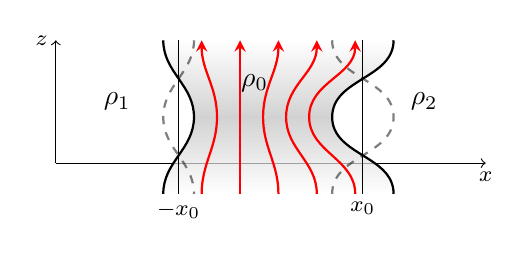
\begin{tikzpicture}[scale=0.78]
				\draw [->] (0,0) -- (7,0);
				
				\shade[bottom color=lightgray,top color=white, opacity=0.7] (1.75,2) to [out=-90,in=90] (2.25,0.75) to (4.5,0.75) to [out=90,in=-90] (5.5,2) to (1.75,2);
				
				\shade[bottom color=white,top color=lightgray, opacity=0.7] (2.25,0.75) to (4.5,0.75) to [out=-90,in=90] (5.5,-0.5) to (1.75,-0.5) to [out=90,in=-90] (2.25,0.75);
				
				\draw [thick] (1.75,2) to [out=-90,in=90] (2.25,0.75) to [out=-90,in=90] (1.75,-0.5);
				\draw [thick, dashed, opacity=0.5] (4.5,2) to [out=-90,in=90] (5.5,0.75) to [out=-90,in=90] (4.5,-0.5);
				
				\draw [thick, red, -stealth] (2.375,-0.5) to [out=90,in=-90] (2.625, 0.75) to [out=90,in=-90] (2.375,2);
				\draw [thick, red, -stealth] (3,-0.5) to [out=90,in=-90] (3, 0.75) to [out=90,in=-90] (3,2);
				\draw [thick, red, -stealth] (3.625,-0.5) to [out=90,in=-90] (3.375, 0.75) to [out=90,in=-90] (3.625,2);
				\draw [thick, red, -stealth] (4.25,-0.5) to [out=90,in=-90] (3.75, 0.75) to [out=90,in=-90] (4.25,2);
				\draw [thick, red, -stealth] (4.875,-0.5) to [out=90,in=-90] (4.125, 0.75) to [out=90,in=-90] (4.875,2);
				
				\draw [thick, dashed, opacity=0.5] (2.25,2) to [out=-90,in=90] (1.75,0.75) to [out=-90,in=90] (2.25,-0.5);
				\draw [thick] (5.5,2) to [out=-90,in=90] (4.5,0.75) to [out=-90,in=90] (5.5,-0.5);
				
				% % % % % % % % % % % % % % % % % % % % % % % % % %
				
				\draw [->] (0,0) -- (0,2);
				
				\node at (1,1) {$\rho_1$};
				\node at (6,1) {$\rho_2$};
				\node [right] at (2.86,1.3) {$\rho_0$};
				
				\footnotesize
				\node [below] at (2,-0.5) {$-x_0$};
				\node [below] at (5,-0.5) {$x_0$};
				
				\node [left] at (0,2) {$z$};
				\node [below] at (7,0) {$x$};
				\draw [-] (2,-0.5) -- (2,2);
				\draw [-] (5,-0.5) -- (5,2);
				\end{tikzpicture}
				\label{fig:kink}}}}
	\caption{Quasi-kink and quasi-sausage modes with external density ordering $\rho_1>\rho_2$. The red lines illustrate the perturbed magnetic field, the thick solid black lines illustrate the perturbed slab boundaries, and the dashed lines illustrate the future position of the slab boundaries after half a period.}
\end{figure} 

The surface and body properties also take a modified form in an asymmetric slab. For a surface mode (for visualisation see Figures~\ref{fig:surf quasi-kink} and~\ref{fig:surf quasi-saus}), the wave power distribution across the slab has a single minimum. The displacement of this minimum from the centre of the slab is a consequence of the asymmetry in the external plasma. The intensity of the maximum amplitudes on the left and right boundaries of the slab ($x=\pm{}x_0$) is different, reflecting the asymmetry in the external plasma.

Body modes are also affected by the asymmetric external environment (for visualisation see Figures~\ref{fig:body quasi-kink} and~\ref{fig:body quasi-saus}). Local maxima and minima in wave power are shifted towards the external plasma of higher density for a quasi-kink body mode and towards the external plasma of lower density for a quasi-sausage mode. However, body modes depend only weakly on the external plasma parameters and are less affected than surface modes. This is shown analytically in Sections~\ref{sec:thin} and~\ref{sec:wide}.

\begin{figure}
	\makebox[\textwidth][c]{
		\subfloat[Quasi-kink surface mode]{\scalebox{1}{
				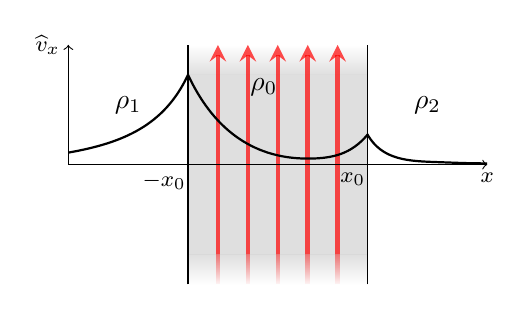
\begin{tikzpicture}[scale=0.76]
				\path [fill=lightgray, opacity=0.5] (2,-1.5) -- (2,1.5) -- (5,1.5) -- (5,-1.5) -- (2,-1.5);
				
				\shade[bottom color=white,top color=lightgray, opacity=0.5] (2,-2) to (5,-2) to (5,-1.5) to (2,-1.5) to (2,-2);
				
				\shade[top color=white,bottom color=lightgray, opacity=0.5] (2,2) to (5,2) to (5,1.5) to (2,1.5) to (2,2);
				
				\draw [-] (2,-2) -- (2,2);
				\draw [-] (5,-2) -- (5,2);
				
				\draw [ultra thick, red, -stealth,opacity=0.7] (2.5,-1.5) -- (2.5,2);
				\draw [ultra thick, red, path fading=south, opacity=0.5] (2.5,-2) -- (2.5,-1.5);
				\draw [ultra thick, red, -stealth,opacity=0.7] (3,-1.5) -- (3,2);
				\draw [ultra thick, red, path fading=south,opacity=0.5] (3,-2) -- (3,-1.5);
				\draw [ultra thick, red, -stealth,opacity=0.7] (3.5,-1.5) -- (3.5,2);
				\draw [ultra thick, red, path fading=south,opacity=0.5] (3.5,-2) -- (3.5,-1.5);
				\draw [ultra thick, red, -stealth,opacity=0.7] (4,-1.5) -- (4,2);
				\draw [ultra thick, red, path fading=south,opacity=0.5] (4,-2) -- (4,-1.5);
				\draw [ultra thick, red, -stealth,opacity=0.7] (4.5,-1.5) -- (4.5,2);
				\draw [ultra thick, red, path fading=south,opacity=0.5] (4.5,-2) -- (4.5,-1.5);
				
				\draw [thick] (0,0.2) to [out=10, in=245] (2, 1.5) to [out=295, in=180] (4,0.1) to [out=0, in=230] (5,0.5) to [out=300, in=178] (6.2,0.04) to [out=358, in=180] (7,0.02);
				
				\draw [->] (0,0) -- (0,2);
				\draw [->] (0,0) -- (7,0);
				
				\node at (1,1) {$\rho_1$};
				\node at (6,1) {$\rho_2$};
				\node [right] at (2.88,1.3) {$\rho_0$};
				
				\footnotesize
				\node [below left] at (2.1,0) {$-x_0$};
				\node [below left] at (5.1,0) {$x_0$};
				
				\node [left] at (0,2) {$\widehat{v}_x$};
				\node [below] at (7,0) {$x$};
				\end{tikzpicture}
				\label{fig:surf quasi-kink}}}
		%
		%
		%
		%
		\subfloat[Quasi-sausage surface mode]{\scalebox{1}{
				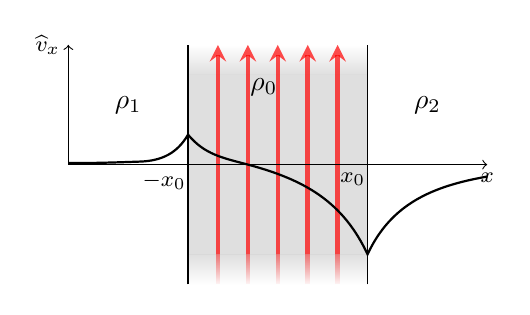
\begin{tikzpicture}[scale=0.76]
				\path [fill=lightgray, opacity=0.5] (2,-1.5) -- (2,1.5) -- (5,1.5) -- (5,-1.5) -- (2,-1.5);
				
				\shade[bottom color=white,top color=lightgray, opacity=0.5] (2,-2) to (5,-2) to (5,-1.5) to (2,-1.5) to (2,-2);
				
				\shade[top color=white,bottom color=lightgray, opacity=0.5] (2,2) to (5,2) to (5,1.5) to (2,1.5) to (2,2);
				
				\draw [-] (2,-2) -- (2,2);
				\draw [-] (5,-2) -- (5,2);
				
				\draw [ultra thick, red, -stealth,opacity=0.7] (2.5,-1.5) -- (2.5,2);
				\draw [ultra thick, red, path fading=south, opacity=0.5] (2.5,-2) -- (2.5,-1.5);
				\draw [ultra thick, red, -stealth,opacity=0.7] (3,-1.5) -- (3,2);
				\draw [ultra thick, red, path fading=south,opacity=0.5] (3,-2) -- (3,-1.5);
				\draw [ultra thick, red, -stealth,opacity=0.7] (3.5,-1.5) -- (3.5,2);
				\draw [ultra thick, red, path fading=south,opacity=0.5] (3.5,-2) -- (3.5,-1.5);
				\draw [ultra thick, red, -stealth,opacity=0.7] (4,-1.5) -- (4,2);
				\draw [ultra thick, red, path fading=south,opacity=0.5] (4,-2) -- (4,-1.5);
				\draw [ultra thick, red, -stealth,opacity=0.7] (4.5,-1.5) -- (4.5,2);
				\draw [ultra thick, red, path fading=south,opacity=0.5] (4.5,-2) -- (4.5,-1.5);
				
				\draw [thick] (0,0.025) to [out=0, in=-178] (1.2, 0.05) to [out=2, in=-120] (2,0.5) to [out=-50, in=165] (3,0) to [out=-15, in=115] (5,-1.5) to [out=65, in=-170] (7,-0.2);
				\draw [->] (0,0) -- (0,2);
				\draw [->] (0,0) -- (7,0);
				
				\node at (1,1) {$\rho_1$};
				\node at (6,1) {$\rho_2$};
				\node [right] at (2.88,1.3) {$\rho_0$};
				
				\footnotesize
				\node [below left] at (2.1,0) {$-x_0$};
				\node [below left] at (5.1,0) {$x_0$};
				
				\node [left] at (0,2) {$\widehat{v}_x$};
				\node [below] at (7,0) {$x$};
				\end{tikzpicture}
				\label{fig:surf quasi-saus}}}}
	%
	%
	\\
	%
	%
	\makebox[\textwidth][c]{
		\subfloat[Quasi-kink body mode]{\scalebox{1}{
				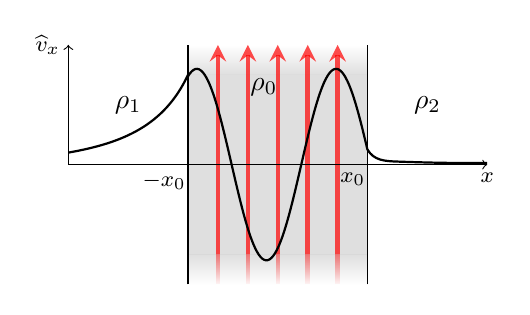
\begin{tikzpicture}[scale=0.76]
				\path [fill=lightgray, opacity=0.5] (2,-1.5) -- (2,1.5) -- (5,1.5) -- (5,-1.5) -- (2,-1.5);
				
				\shade[bottom color=white,top color=lightgray, opacity=0.5] (2,-2) to (5,-2) to (5,-1.5) to (2,-1.5) to (2,-2);
				
				\shade[top color=white,bottom color=lightgray, opacity=0.5] (2,2) to (5,2) to (5,1.5) to (2,1.5) to (2,2);
				
				\draw [-] (2,-2) -- (2,2);
				\draw [-] (5,-2) -- (5,2);
				
				\draw [thick] (7,0.025) to [out=180, in=358] (5.5, 0.05) to [out=178, in=300] (5,0.25);
				
				
				\draw [ultra thick, red, -stealth,opacity=0.7] (2.5,-1.5) -- (2.5,2);
				\draw [ultra thick, red, path fading=south, opacity=0.5] (2.5,-2) -- (2.5,-1.5);
				\draw [ultra thick, red, -stealth,opacity=0.7] (3,-1.5) -- (3,2);
				\draw [ultra thick, red, path fading=south,opacity=0.5] (3,-2) -- (3,-1.5);
				\draw [ultra thick, red, -stealth,opacity=0.7] (3.5,-1.5) -- (3.5,2);
				\draw [ultra thick, red, path fading=south,opacity=0.5] (3.5,-2) -- (3.5,-1.5);
				\draw [ultra thick, red, -stealth,opacity=0.7] (4,-1.5) -- (4,2);
				\draw [ultra thick, red, path fading=south,opacity=0.5] (4,-2) -- (4,-1.5);
				\draw [ultra thick, red, -stealth,opacity=0.7] (4.5,-1.5) -- (4.5,2);
				\draw [ultra thick, red, path fading=south,opacity=0.5] (4.5,-2) -- (4.5,-1.5);
				
				\draw [thick, smooth, samples=100, domain=2:5] plot (\x,{1.6*cos(2.7*(\x+0.18) r)});
				
				\draw [thick] (0,0.2) to [out=10, in=245] (2, 1.5);
				
				\draw [->] (0,0) -- (0,2);
				\draw [->] (0,0) -- (7,0);
				
				\node at (1,1) {$\rho_1$};
				\node at (6,1) {$\rho_2$};
				\node [right] at (2.88,1.3) {$\rho_0$};
				
				\footnotesize
				\node [below left] at (2.1,0) {$-x_0$};
				\node [below left] at (5.1,0) {$x_0$};
				
				\node [left] at (0,2) {$\widehat{v}_x$};
				\node [below] at (7,0) {$x$};
				\end{tikzpicture}
				\label{fig:body quasi-kink}}}
		%
		%
		%
		%
		\subfloat[Quasi-sausage body mode]{\scalebox{1}{
				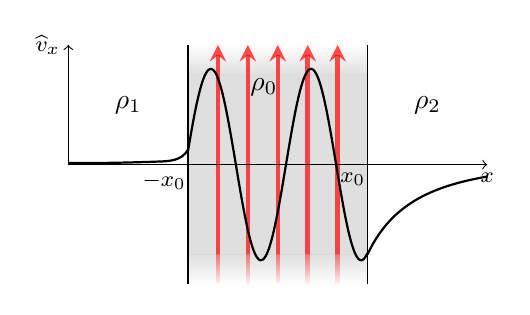
\begin{tikzpicture}[scale=0.76]
				\path [fill=lightgray, opacity=0.5] (2,-1.5) -- (2,1.5) -- (5,1.5) -- (5,-1.5) -- (2,-1.5);
				
				\shade[bottom color=white,top color=lightgray, opacity=0.5] (2,-2) to (5,-2) to (5,-1.5) to (2,-1.5) to (2,-2);
				
				\shade[top color=white,bottom color=lightgray, opacity=0.5] (2,2) to (5,2) to (5,1.5) to (2,1.5) to (2,2);
				
				\draw [-] (2,-2) -- (2,2);
				\draw [-] (5,-2) -- (5,2);
				
				\draw [thick] (0,0.025) to [out=0, in=-178] (1.5, 0.05) to [out=2, in=-120] (2,0.25);
				
				\draw [ultra thick, red, -stealth,opacity=0.7] (2.5,-1.5) -- (2.5,2);
				\draw [ultra thick, red, path fading=south, opacity=0.5] (2.5,-2) -- (2.5,-1.5);
				\draw [ultra thick, red, -stealth,opacity=0.7] (3,-1.5) -- (3,2);
				\draw [ultra thick, red, path fading=south,opacity=0.5] (3,-2) -- (3,-1.5);
				\draw [ultra thick, red, -stealth,opacity=0.7] (3.5,-1.5) -- (3.5,2);
				\draw [ultra thick, red, path fading=south,opacity=0.5] (3.5,-2) -- (3.5,-1.5);
				\draw [ultra thick, red, -stealth,opacity=0.7] (4,-1.5) -- (4,2);
				\draw [ultra thick, red, path fading=south,opacity=0.5] (4,-2) -- (4,-1.5);
				\draw [ultra thick, red, -stealth,opacity=0.7] (4.5,-1.5) -- (4.5,2);
				\draw [ultra thick, red, path fading=south,opacity=0.5] (4.5,-2) -- (4.5,-1.5);
				
				%\draw [thick] (2,0.5) to [out=-50, in=180] (2.3,0.25) to [out=0, in=180] (3.2,1) to [out=0, in=180] (4.1,0.1) to [out=-0, in=-120] (5,1.5);
				
				\draw [thick, smooth, samples=100, domain=2:5] plot (\x,{1.6*cos(3.75*(\x-0.705) r)});
				
				\draw [thick] (5,-1.5) to [out=65, in=-170] (7,-0.2);
				
				\draw [->] (0,0) -- (0,2);
				\draw [->] (0,0) -- (7,0);
				
				\node at (1,1) {$\rho_1$};
				\node at (6,1) {$\rho_2$};
				\node [right] at (2.88,1.3) {$\rho_0$};
				
				\footnotesize
				\node [below left] at (2.1,0) {$-x_0$};
				\node [below left] at (5.1,0) {$x_0$};
				
				\node [left] at (0,2) {$\widehat{v}_x$};
				\node [below] at (7,0) {$x$};
				\end{tikzpicture}
				\label{fig:body quasi-saus}}}}
	\caption{The transverse velocity perturbation amplitude, $\widehat{v}_x$ as a function of the transverse spatial coordinate, $x$, for quasi-sausage and quasi-kink modes in an isolated magnetic slab with external density ordering $\rho_1 > \rho_2$.}
\end{figure}


%------------------------------------------------------------------------------
\section{Asymmetric slab in a non-magnetic environment}
\label{sec: EVP non-mag}
%------------------------------------------------------------------------------

Much of the interesting physics due to waveguide asymmetry is exhibited by a magnetic slab with non-magnetic external plasma. We study this system in this Section.

By letting $B_1 = B_2 = 0$, the plasma in the external regions is non-magnetic. Then the dispersion relation, Equation~\eqref{DR}, simplifies slightly to
\begin{align}
&m_0^2\omega^4 + \frac{\rho_0}{\rho_1}m_1\frac{\rho_0}{\rho_2}m_2(k^2v_\textrm{A0}^2 - \omega^2)^2 \notag \\
& - m_0(k^2v_{A0}^2 - \omega^2)\left[\frac{\rho_0}{\rho_1}m_1 + \frac{\rho_0}{\rho_2}m_2\right]\coth{2m_0x_0} = 0, \label{DR non-mag}
\end{align}
and the dispersion relation for an approximately symmetric slab simplifies slightly to
\begin{equation}
(k^2v_\textrm{A0}^2-\omega^2)\left(\frac{\rho_0}{\rho_1}m_1 + \frac{\rho_0}{\rho_2}m_2\right) = 2\omega^2m_0\left(\begin{matrix}\tanh \\ \coth \end{matrix}\right)(m_0x_0) = 0. \label{DRapprox non-mag}
\end{equation}


\subsection{Analytical solutions}


The full dispersion relation, Equation~\eqref{DRapprox non-mag} does not allow for 


\subsubsection{Spurious solutions}

\subsubsection{Limiting case - incompressible plasma}

\subsubsection{Limiting case - zero-beta}

\subsubsection{Limiting case - thin slab}

\subsubsection{Limiting case - wide slab}

\subsection{Numerical solutions}

\subsubsection{Varying the degree of asymmetry}

\subsection{Analogy to coupled spring and mass oscillator}
Actually do the maths for this.


%------------------------------------------------------------------------------
\section{Asymmetric slab in a magnetic environment}
\label{sec: EVP mag}
%------------------------------------------------------------------------------

\subsection{Model description}

\subsection{The dispersion relation}

\subsection{Implications for observations}

\subsubsection{Quasi-symmetric modes}

\subsubsection{Asymmetric mode or superposition of symmetric modes?}
Table of observable indicators of each case.

\subsubsection{Possible alternative causes of observed asymmetry}
Possibilities: 
\begin{itemize}
	\item Asymmetric ICs
	\item Non-collective oscillations
	\item Observational artefact
\end{itemize}
Include discussion about how to differentiate between these.



\bibliographystyle{plainnat}
\bibliography{../main/references}  

\end{document}
